% Options for packages loaded elsewhere
\PassOptionsToPackage{unicode}{hyperref}
\PassOptionsToPackage{hyphens}{url}
\PassOptionsToPackage{dvipsnames,svgnames,x11names}{xcolor}
%
\documentclass[
  letterpaper,
  DIV=11,
  numbers=noendperiod]{scrartcl}

\usepackage{amsmath,amssymb}
\usepackage{iftex}
\ifPDFTeX
  \usepackage[T1]{fontenc}
  \usepackage[utf8]{inputenc}
  \usepackage{textcomp} % provide euro and other symbols
\else % if luatex or xetex
  \usepackage{unicode-math}
  \defaultfontfeatures{Scale=MatchLowercase}
  \defaultfontfeatures[\rmfamily]{Ligatures=TeX,Scale=1}
\fi
\usepackage{lmodern}
\ifPDFTeX\else  
    % xetex/luatex font selection
\fi
% Use upquote if available, for straight quotes in verbatim environments
\IfFileExists{upquote.sty}{\usepackage{upquote}}{}
\IfFileExists{microtype.sty}{% use microtype if available
  \usepackage[]{microtype}
  \UseMicrotypeSet[protrusion]{basicmath} % disable protrusion for tt fonts
}{}
\makeatletter
\@ifundefined{KOMAClassName}{% if non-KOMA class
  \IfFileExists{parskip.sty}{%
    \usepackage{parskip}
  }{% else
    \setlength{\parindent}{0pt}
    \setlength{\parskip}{6pt plus 2pt minus 1pt}}
}{% if KOMA class
  \KOMAoptions{parskip=half}}
\makeatother
\usepackage{xcolor}
\setlength{\emergencystretch}{3em} % prevent overfull lines
\setcounter{secnumdepth}{-\maxdimen} % remove section numbering
% Make \paragraph and \subparagraph free-standing
\makeatletter
\ifx\paragraph\undefined\else
  \let\oldparagraph\paragraph
  \renewcommand{\paragraph}{
    \@ifstar
      \xxxParagraphStar
      \xxxParagraphNoStar
  }
  \newcommand{\xxxParagraphStar}[1]{\oldparagraph*{#1}\mbox{}}
  \newcommand{\xxxParagraphNoStar}[1]{\oldparagraph{#1}\mbox{}}
\fi
\ifx\subparagraph\undefined\else
  \let\oldsubparagraph\subparagraph
  \renewcommand{\subparagraph}{
    \@ifstar
      \xxxSubParagraphStar
      \xxxSubParagraphNoStar
  }
  \newcommand{\xxxSubParagraphStar}[1]{\oldsubparagraph*{#1}\mbox{}}
  \newcommand{\xxxSubParagraphNoStar}[1]{\oldsubparagraph{#1}\mbox{}}
\fi
\makeatother

\usepackage{color}
\usepackage{fancyvrb}
\newcommand{\VerbBar}{|}
\newcommand{\VERB}{\Verb[commandchars=\\\{\}]}
\DefineVerbatimEnvironment{Highlighting}{Verbatim}{commandchars=\\\{\}}
% Add ',fontsize=\small' for more characters per line
\usepackage{framed}
\definecolor{shadecolor}{RGB}{241,243,245}
\newenvironment{Shaded}{\begin{snugshade}}{\end{snugshade}}
\newcommand{\AlertTok}[1]{\textcolor[rgb]{0.68,0.00,0.00}{#1}}
\newcommand{\AnnotationTok}[1]{\textcolor[rgb]{0.37,0.37,0.37}{#1}}
\newcommand{\AttributeTok}[1]{\textcolor[rgb]{0.40,0.45,0.13}{#1}}
\newcommand{\BaseNTok}[1]{\textcolor[rgb]{0.68,0.00,0.00}{#1}}
\newcommand{\BuiltInTok}[1]{\textcolor[rgb]{0.00,0.23,0.31}{#1}}
\newcommand{\CharTok}[1]{\textcolor[rgb]{0.13,0.47,0.30}{#1}}
\newcommand{\CommentTok}[1]{\textcolor[rgb]{0.37,0.37,0.37}{#1}}
\newcommand{\CommentVarTok}[1]{\textcolor[rgb]{0.37,0.37,0.37}{\textit{#1}}}
\newcommand{\ConstantTok}[1]{\textcolor[rgb]{0.56,0.35,0.01}{#1}}
\newcommand{\ControlFlowTok}[1]{\textcolor[rgb]{0.00,0.23,0.31}{\textbf{#1}}}
\newcommand{\DataTypeTok}[1]{\textcolor[rgb]{0.68,0.00,0.00}{#1}}
\newcommand{\DecValTok}[1]{\textcolor[rgb]{0.68,0.00,0.00}{#1}}
\newcommand{\DocumentationTok}[1]{\textcolor[rgb]{0.37,0.37,0.37}{\textit{#1}}}
\newcommand{\ErrorTok}[1]{\textcolor[rgb]{0.68,0.00,0.00}{#1}}
\newcommand{\ExtensionTok}[1]{\textcolor[rgb]{0.00,0.23,0.31}{#1}}
\newcommand{\FloatTok}[1]{\textcolor[rgb]{0.68,0.00,0.00}{#1}}
\newcommand{\FunctionTok}[1]{\textcolor[rgb]{0.28,0.35,0.67}{#1}}
\newcommand{\ImportTok}[1]{\textcolor[rgb]{0.00,0.46,0.62}{#1}}
\newcommand{\InformationTok}[1]{\textcolor[rgb]{0.37,0.37,0.37}{#1}}
\newcommand{\KeywordTok}[1]{\textcolor[rgb]{0.00,0.23,0.31}{\textbf{#1}}}
\newcommand{\NormalTok}[1]{\textcolor[rgb]{0.00,0.23,0.31}{#1}}
\newcommand{\OperatorTok}[1]{\textcolor[rgb]{0.37,0.37,0.37}{#1}}
\newcommand{\OtherTok}[1]{\textcolor[rgb]{0.00,0.23,0.31}{#1}}
\newcommand{\PreprocessorTok}[1]{\textcolor[rgb]{0.68,0.00,0.00}{#1}}
\newcommand{\RegionMarkerTok}[1]{\textcolor[rgb]{0.00,0.23,0.31}{#1}}
\newcommand{\SpecialCharTok}[1]{\textcolor[rgb]{0.37,0.37,0.37}{#1}}
\newcommand{\SpecialStringTok}[1]{\textcolor[rgb]{0.13,0.47,0.30}{#1}}
\newcommand{\StringTok}[1]{\textcolor[rgb]{0.13,0.47,0.30}{#1}}
\newcommand{\VariableTok}[1]{\textcolor[rgb]{0.07,0.07,0.07}{#1}}
\newcommand{\VerbatimStringTok}[1]{\textcolor[rgb]{0.13,0.47,0.30}{#1}}
\newcommand{\WarningTok}[1]{\textcolor[rgb]{0.37,0.37,0.37}{\textit{#1}}}

\providecommand{\tightlist}{%
  \setlength{\itemsep}{0pt}\setlength{\parskip}{0pt}}\usepackage{longtable,booktabs,array}
\usepackage{calc} % for calculating minipage widths
% Correct order of tables after \paragraph or \subparagraph
\usepackage{etoolbox}
\makeatletter
\patchcmd\longtable{\par}{\if@noskipsec\mbox{}\fi\par}{}{}
\makeatother
% Allow footnotes in longtable head/foot
\IfFileExists{footnotehyper.sty}{\usepackage{footnotehyper}}{\usepackage{footnote}}
\makesavenoteenv{longtable}
\usepackage{graphicx}
\makeatletter
\def\maxwidth{\ifdim\Gin@nat@width>\linewidth\linewidth\else\Gin@nat@width\fi}
\def\maxheight{\ifdim\Gin@nat@height>\textheight\textheight\else\Gin@nat@height\fi}
\makeatother
% Scale images if necessary, so that they will not overflow the page
% margins by default, and it is still possible to overwrite the defaults
% using explicit options in \includegraphics[width, height, ...]{}
\setkeys{Gin}{width=\maxwidth,height=\maxheight,keepaspectratio}
% Set default figure placement to htbp
\makeatletter
\def\fps@figure{htbp}
\makeatother

\KOMAoption{captions}{tableheading}
\makeatletter
\@ifpackageloaded{caption}{}{\usepackage{caption}}
\AtBeginDocument{%
\ifdefined\contentsname
  \renewcommand*\contentsname{Table of contents}
\else
  \newcommand\contentsname{Table of contents}
\fi
\ifdefined\listfigurename
  \renewcommand*\listfigurename{List of Figures}
\else
  \newcommand\listfigurename{List of Figures}
\fi
\ifdefined\listtablename
  \renewcommand*\listtablename{List of Tables}
\else
  \newcommand\listtablename{List of Tables}
\fi
\ifdefined\figurename
  \renewcommand*\figurename{Figure}
\else
  \newcommand\figurename{Figure}
\fi
\ifdefined\tablename
  \renewcommand*\tablename{Table}
\else
  \newcommand\tablename{Table}
\fi
}
\@ifpackageloaded{float}{}{\usepackage{float}}
\floatstyle{ruled}
\@ifundefined{c@chapter}{\newfloat{codelisting}{h}{lop}}{\newfloat{codelisting}{h}{lop}[chapter]}
\floatname{codelisting}{Listing}
\newcommand*\listoflistings{\listof{codelisting}{List of Listings}}
\makeatother
\makeatletter
\makeatother
\makeatletter
\@ifpackageloaded{caption}{}{\usepackage{caption}}
\@ifpackageloaded{subcaption}{}{\usepackage{subcaption}}
\makeatother

\ifLuaTeX
  \usepackage{selnolig}  % disable illegal ligatures
\fi
\usepackage{bookmark}

\IfFileExists{xurl.sty}{\usepackage{xurl}}{} % add URL line breaks if available
\urlstyle{same} % disable monospaced font for URLs
\hypersetup{
  pdftitle={Basic ERGM estimation},
  pdfauthor={Simone Santoni},
  colorlinks=true,
  linkcolor={blue},
  filecolor={Maroon},
  citecolor={Blue},
  urlcolor={Blue},
  pdfcreator={LaTeX via pandoc}}


\title{Basic ERGM estimation}
\author{Simone Santoni}
\date{2024-11-19}

\begin{document}
\maketitle
\begin{abstract}
This notebook shows how to fit a basic ERGM on a one-mode, directed
network dataset
\end{abstract}


\section{Notebook setup}\label{notebook-setup}

\subsection{Load libraries}\label{load-libraries}

We need to load three libraries:

\begin{itemize}
\tightlist
\item
  \href{https://cran.r-project.org/web/packages/car/car.pdf}{\texttt{car}},
  which stands for `Companion to Applied Regression,' provides utility
  functions regarding regression models
\item
  \href{https://cran.r-project.org/web/packages/sna/index.html}{\texttt{sna}},
  a \href{https://statnet.org/}{Statnet}'s library, includes many
  network descriptives
\item
  \href{}{\texttt{ergm}}, another \href{https://statnet.org/}{Statnet}'s
  library, implements ERGMs.
\end{itemize}

\begin{Shaded}
\begin{Highlighting}[]
\FunctionTok{library}\NormalTok{(car)}
\FunctionTok{library}\NormalTok{(sna)}
\FunctionTok{library}\NormalTok{(ergm)}
\end{Highlighting}
\end{Shaded}

\subsection{Load data}\label{load-data}

\section{ERGM 101}\label{ergm-101}

\textbf{What is the objective of ERGMs?}

ERGMs test how and to what extent an observed network exhibits certain
tie formation mechanisms. Example of tie formation mechanisms include
(but they are not limited to):

\begin{itemize}
\tightlist
\item
  In-degree centrality, the tendency of a node \(i\) to receive ties
\item
  Out-degree centrality, the tendency of a node \(i\) to send ties
\item
  Reciprocity, a \emph{dyadic} tendency such that \(i \rightarrow j\) \&
  \(j \rightarrow i\)
\item
  Transitive closure, a \emph{triadic} tendency such that i.e.,
  \(i \rightarrow j\) \& \(j \rightarrow w\) \& \(i \rightarrow w\)
\item
  Balance, the tendency for two nodes \(i\) and \(j\) to share alters
  \(a = {a_{1}, a_{2}, ..., a_{n}}\)
\item
  Node attributes, i.e., node \(i\)'s qualities
\item
  Dyadic attributes, i.e., the similarity (or differences) in nodes
  \(i\) and \(j\) qualities
\end{itemize}

\textbf{What is the intuition behind ERGMs?}

ERGMs consider observed networks as mixtures of network effects

\subsection{The General Form of ERGM}\label{the-general-form-of-ergm}

ERGMs estimate the probabilities that the observed network \(y\) comes
from the class \(Y\) based on a set of endogenous and exogenous tie
formation explanations (aka `model effects'). ERGM's general form is the
following:

\begin{equation}\label{eq:ergm_gen_form}
Pr(Y = y|X) = \frac{exp[\theta^{T}g(y,X)]}{k(\theta)}
\end{equation}

where \(\theta^{T}\) is the vector of regression coefficients regarding
the model effects \(g(y, X)\), and \(k(\theta)\) is the summation of the
numerator's value over the set of all possible networks \(y\).

To better understand ERGM's general form, we can dispense the numerator
of the previous equation as follows:

\begin{equation}
  [\theta_{1}, \theta_{2}, ..., \theta_{n}]\begin{bmatrix}
           g_{1}(y) \\
           g_{2}(y) \\
           \vdots \\
           g_{n}(y)
        \end{bmatrix}
        = \sum_{i=1}^{n} \theta_{i} \cdot g_{i}(y)
  \end{equation}

This equation highlights that the probability of observing a particular
network in a set of networks―e.g., ten-node networks exhibiting
significant in-degree popularity and reciprocity―as a function of many
\(g(y)\). We can also dispense the equation in terms of the log odds of
an edge:

\begin{equation}
logit(Y_{ij} = 1) = \theta^{T} \cdot \delta[g(y, X)]_{ij}
\end{equation}

where \(\delta[(y, X)]\) is the `change' statistic, that is, the change
in \(g(y,X)\) when the value of only the \(ij\) dyad is changed from 0
to 1.

\subsection{Examples of Model Effects}\label{examples-of-model-effects}

\begin{figure}

\begin{minipage}{\linewidth}

\centering{

\pandocbounded{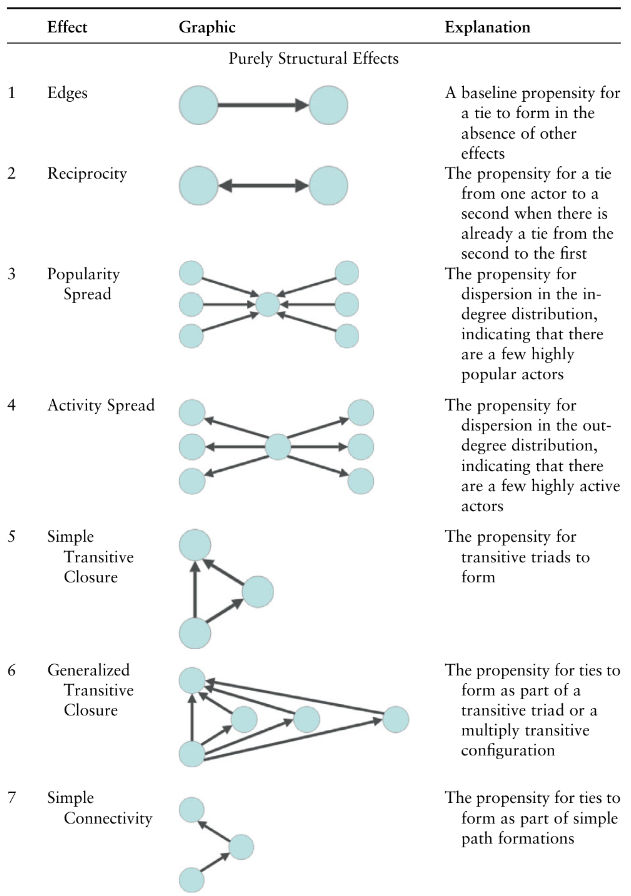
\includegraphics[keepaspectratio]{imgs/model_effects_1.png}}

}

\subcaption{\label{fig-A}}

\end{minipage}%
\newline
\begin{minipage}{\linewidth}

\centering{

\pandocbounded{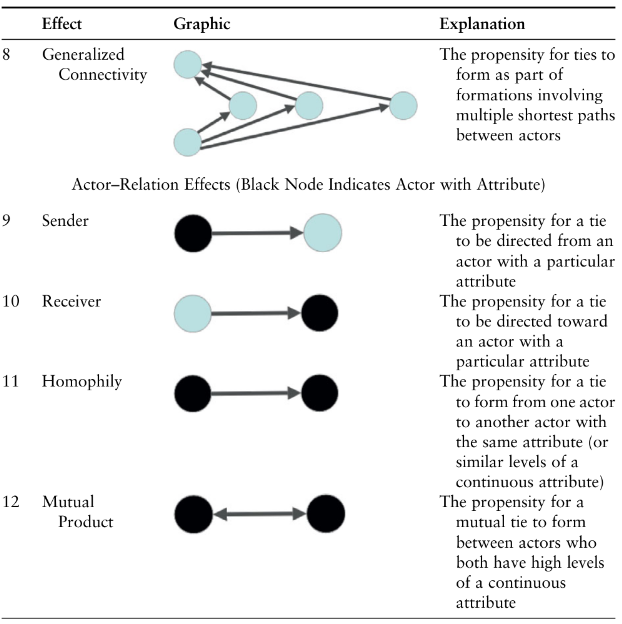
\includegraphics[keepaspectratio]{imgs/model_effects_2.png}}

}

\subcaption{\label{fig-B}}

\end{minipage}%

\caption{\label{fig-model-effects}Model Effects reported in
\href{https://www.cambridge.org/core/books/network-analysis/C9202FD5420BE99225FEED4B6214DBB7}{Rawlings
et al.~(2023, pp.~322-323)}}

\end{figure}%

\subsection{\texorpdfstring{How Do I Compute the Change Statistic
\(\delta[g(y, X)]\)?}{How Do I Compute the Change Statistic \textbackslash delta{[}g(y, X){]}?}}\label{how-do-i-compute-the-change-statistic-deltagy-x}

ERGM libraries, like R's \texttt{ergm}, do that for you. However, it is
important that you familiarize yourself with computing the change
statistic \(\delta[g(y, X)]\). Here are two key premises:

\begin{itemize}
\tightlist
\item
  Mainly, the procedure aims to create the regressors for the
  above-displayed Logit model. For example, one may want to regress the
  likelihood to observe a tie from \(i\) to \(j\) against \(i\) and/or
  \(j\)'s degree, the existence of the tie from \(j\) to \(i\), the fact
  that \(i\) and \(j\) are involved in a triad to which a third node
  \(w\), and so on and so forth
\item
  Overall, the procedure consists of a `thought experiment.' For each
  tie involving a pair of nodes \(\{i, j\}\), we ask ourselves:

  \begin{itemize}
  \tightlist
  \item
    ``Does adding the tie from \(i\) to \(j\) make the relationship
    `reciprocal', that is, \(i \rightarrow j\) \& \(j \rightarrow i\)?''
  \item
    ``Does adding the tie from \(i\) to \(j\) make the triad involving
    \(i\), \(j\), and \(w\) transitive?''
  \item
    ``Is the tie from \(i\) to \(j\) involving two similar (equivalent)
    or dissimilar (different) nodes''
  \end{itemize}
\end{itemize}

The below-displayed figure illustrates this kind of thought experiment
visually. The algorithm will replicate the thought experiment for us,
iterating over all possible pairs of node \$\{i, j\} creating the input
for the Logit regression. The final dataset will have \(N \cdot (N -1)\)
rows (aka ties) and \(K + 1\) columns, where \(K\) is the number of
selected model effects. The \(+ 1\) signifies the column with the
dependent variable information (aka, whether a tie is present or
absent).

\begin{figure}

\centering{

\pandocbounded{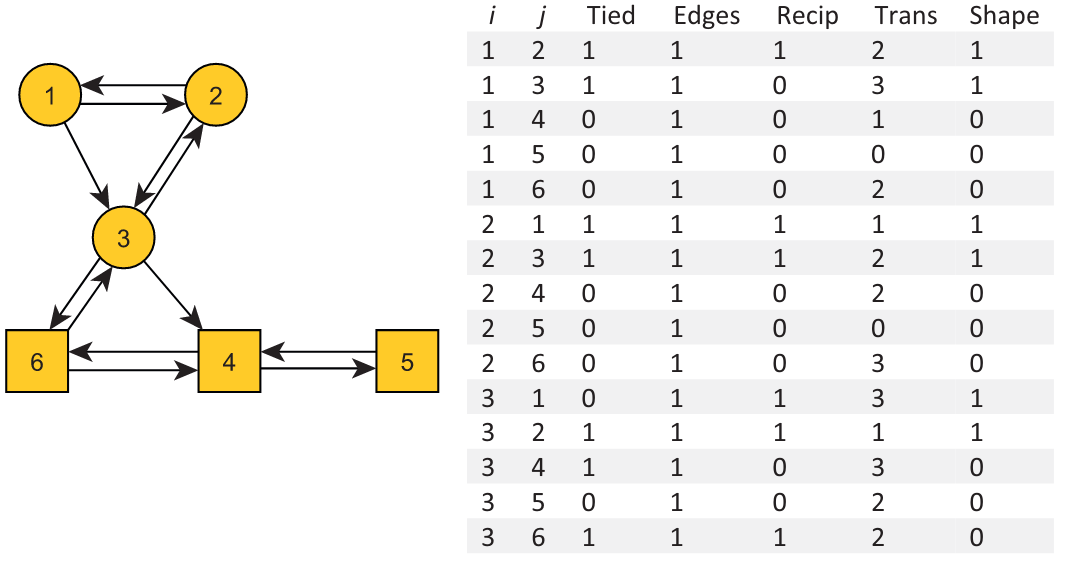
\includegraphics[keepaspectratio]{imgs/thought_exp.png}}

}

\caption{\label{fig-thought-exp}Thought experiments regarding the impact
of \(i \rightarrow j\) on model effects. Source is
\href{https://www.cambridge.org/core/books/network-analysis/C9202FD5420BE99225FEED4B6214DBB7}{Rawlings
et al.~(2023, p.~320)}}

\end{figure}%

\section{Arrange network data}\label{arrange-network-data}

\section{ERGM estimation}\label{ergm-estimation}




\end{document}
